\chapter{Graph Exploration and Structural Insights}
\label{chap:graph_exploration}

\section{Why Explore the Graph Before Prediction?}

It is tempting to treat the graph built in Chapter~\ref{chap:kg} as a black box, but that view is wrong for two reasons. First, \emph{the graph is the dataset}: whether the model's accuracy is driven by genuine cross-case reasoning or by a few dominant hub statutes, whether the five domains are really five or mostly one, and whether the per-case subgraph has the connectivity a message-passing layer needs cannot be answered from prediction results alone. Second, \emph{leakage-safety claims are structural claims}: the leakage-prevention strategy of Section~\ref{sec:leakage_prevention} is only as convincing as the structural evidence that the remaining graph is still dense enough to support learning.

\section{Graph Statistics and Structural Analysis}
\label{sec:graph_stats}

\subsection{Overall Graph Statistics}

The final cross-bucket graph contains \textbf{880{,}176 nodes} and \textbf{1{,}977{,}295 edges}. Average node degree is \textbf{4.49}; the maximum is \textbf{29{,}602}, attained by the \textsc{IPC} statute node.

\begin{table}[H]
  \centering
  \small
  \begin{adjustbox}{max width=\textwidth}
  \begin{tabular}{lrrr}
    \toprule
    Bucket & Cases & Nodes & Edges \\
    \midrule
    Family \& Matrimonial & 15{,}307 & 97{,}150 & 3{,}660{,}068 \\
    Financial Fraud & 14{,}616 & 113{,}240 & 7{,}869{,}952 \\
    Land \& Property & 14{,}052 & 126{,}962 & 9{,}210{,}612 \\
    Motor Accidents & 15{,}237 & 125{,}234 & 7{,}165{,}461 \\
    Sexual Offences & 14{,}597 & 106{,}662 & 7{,}123{,}225 \\
    \midrule
    \textbf{Cross-bucket unified} & \textbf{73{,}809} & \textbf{485{,}540} & \textbf{27{,}243{,}141} \\
    \bottomrule
  \end{tabular}
  \end{adjustbox}
  \caption{Per-bucket and cross-bucket graph statistics. The cross-bucket graph is denser than the sum of per-bucket graphs because shared \textsc{Statute}, \textsc{Provision}, and \textsc{Precedent} nodes acquire edges from every citing bucket.}
  \label{tab:graph_stats}
\end{table}

Family-matrimonial is sparsest by edges-per-case ($\approx 239$); land-property is densest ($\approx 655$), driven by the number of distinct provisions and precedents cited per case.

\subsection{Node Type Distribution}

The node-type breakdown is strongly skewed towards parties and precedents: \textsc{Precedent} (29.0\%), \textsc{Respondent} (21.8\%), \textsc{Petitioner} (19.4\%), with \textsc{Case} (8.3\%), \textsc{Lawyer} (8.4\%), \textsc{Provision} (4.9\%), \textsc{Court} (4.4\%), \textsc{Statute} (2.5\%), \textsc{Judge} (1.3\%) filling out the remainder.

Figure~\ref{fig:shared_vs_local} splits these into shared vs.\ local nodes per bucket. Party nodes are almost entirely local --- a petitioner in one matter rarely recurs in another. Statutes, provisions, courts, and frequently-cited precedents form a small but densely shared layer through which all cross-case message passing flows. Removing party nodes from the shared layer (as the leakage-safe design does) does not destroy cross-case connectivity: the statute and precedent layer remains intact and is the genuine information carrier.

\begin{figure}[H]
  \centering
  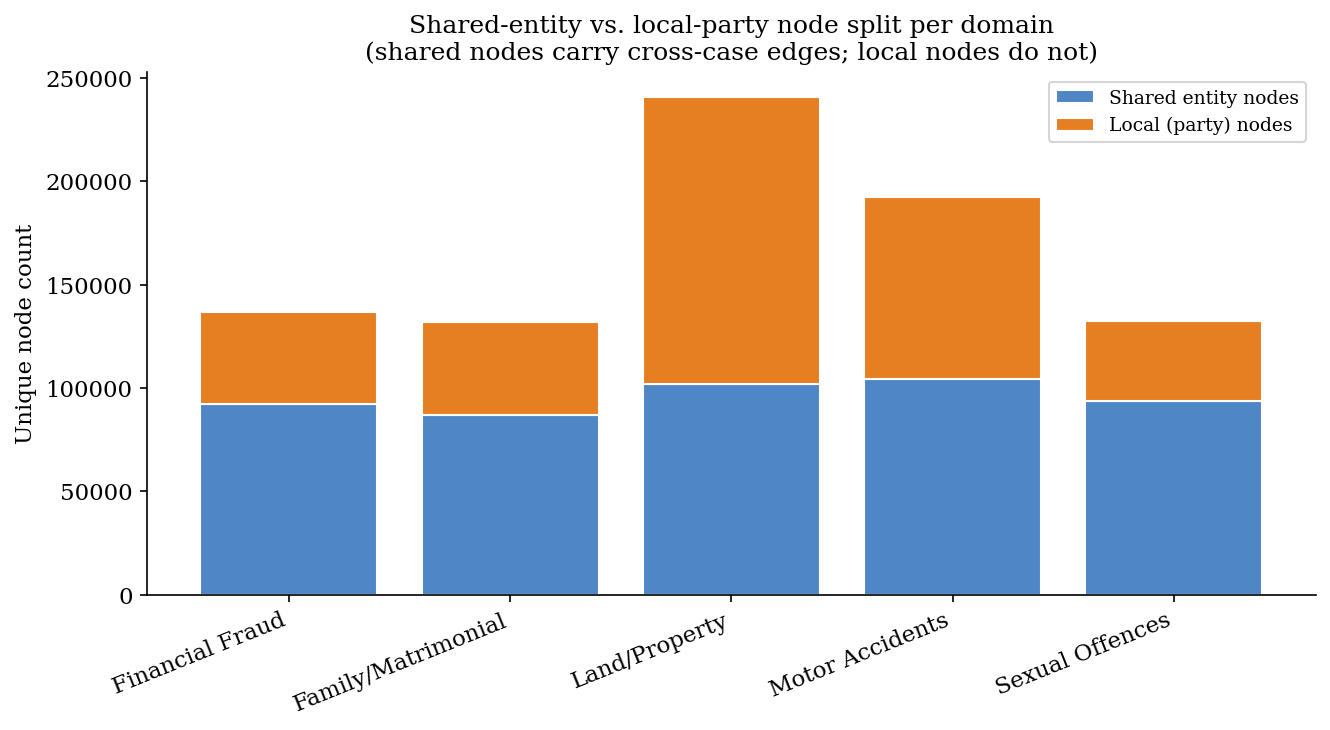
\includegraphics[width=0.92\textwidth]{figures/41_shared_vs_local_nodes_per_bucket.png}
  \caption{Shared vs.\ local node counts per bucket. Party nodes are almost entirely local; statutes, provisions, courts, and frequently-cited precedents form the shared layer.}
  \label{fig:shared_vs_local}
\end{figure}

\subsection{Degree Distribution and Hub Entities}

The top-12 nodes by degree are all statutes, provisions, or courts --- exactly the node types the schema shares across cases:

\begin{table}[H]
  \centering
  \small
  \begin{adjustbox}{max width=\textwidth}
  \begin{tabular}{llrr}
    \toprule
    Node & Type & Degree & Buckets bridged \\
    \midrule
    IPC                                   & Statute   & 29{,}602 & 5 \\
    CR.P.C.                               & Statute   & 18{,}704 & 5 \\
    Supreme Court                         & Court     & 17{,}294 & 5 \\
    Apex Court                            & Court     & 14{,}242 & 5 \\
    Indian Penal Code                     & Statute   & 12{,}009 & 5 \\
    High Court of Judicature at Allahabad & Court     &  8{,}833 & 5 \\
    Section 482                           & Provision &  8{,}732 & 5 \\
    Section 506                           & Provision &  8{,}258 & 5 \\
    I.P.C.                                & Statute   &  7{,}051 & 5 \\
    Section 420                           & Provision &  6{,}285 & 5 \\
    Section 323                           & Provision &  6{,}002 & 5 \\
    Constitution of India                 & Statute   &  5{,}950 & 5 \\
    \bottomrule
  \end{tabular}
  \end{adjustbox}
  \caption{Top hub entities by degree, with the number of buckets they bridge. Every top-12 hub appears in all five domains.}
  \label{tab:top_hubs}
\end{table}

PageRank tells the same story (IPC $0.0114$, Supreme Court $0.0082$, CR.P.C.\ $0.0069$, Apex Court $0.0067$). Figure~\ref{fig:degree_ccdf} confirms the degree distribution is heavy-tailed: most nodes sit at degree one or two while a thin upper tail reaches tens of thousands. The cross-case reasoning capacity of the GNN is therefore structurally concentrated in a handful of statute and court nodes.

\begin{figure}[H]
  \centering
  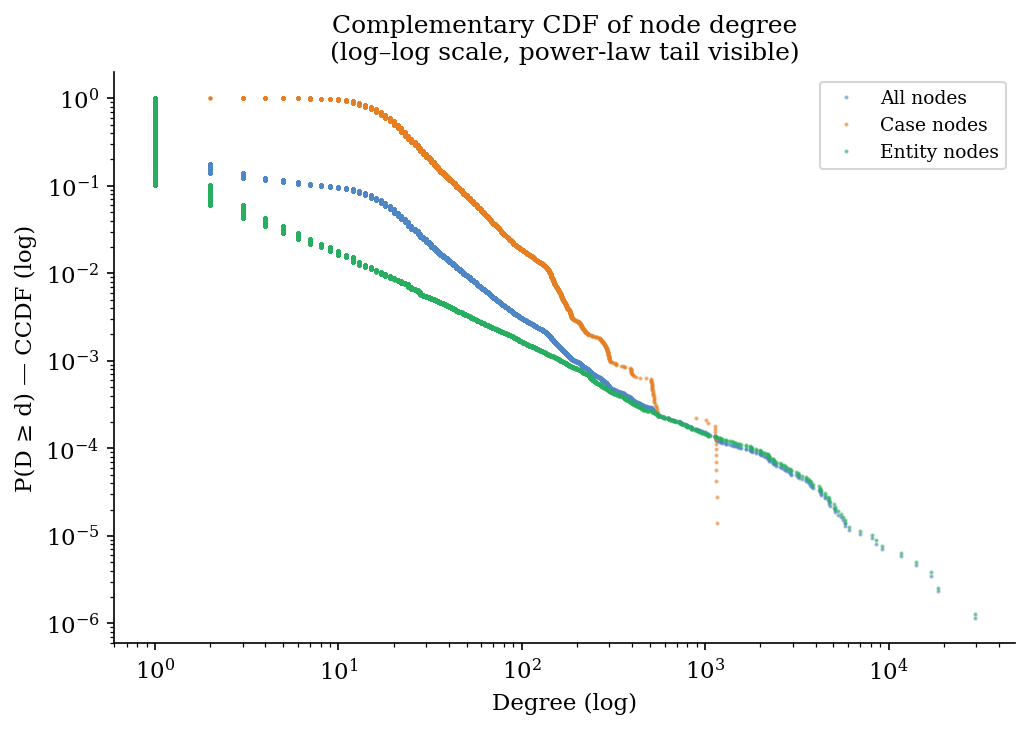
\includegraphics[width=0.92\textwidth]{figures/37_degree_ccdf_loglog.png}
  \caption{Complementary cumulative degree distribution (log-log). Approximately linear decay --- the hallmark of a heavy-tailed, scale-free-like distribution.}
  \label{fig:degree_ccdf}
\end{figure}

\subsection{Cross-Bucket Entity Sharing}

Knowing which individual nodes are hubs is useful; knowing how many entities are shared between each pair of domains is complementary. Figure~\ref{fig:cross_bucket_sharing_matrix} shows three patterns: (i) strong pairwise sharing among Family \& Matrimonial, Financial Fraud, and Sexual Offences (all IPC/CrPC-driven); (ii) moderate sharing between those three and Motor Accidents via general procedural statutes; (iii) weaker sharing with Land \& Property, anchored by its own statutory backbone (Land Acquisition Act, Constitution of India). The domains are related enough for joint training to carry signal but different enough that each keeps its own statutory fingerprint --- motivating a unified cross-bucket graph rather than five separate per-domain graphs.

\begin{figure}[H]
  \centering
  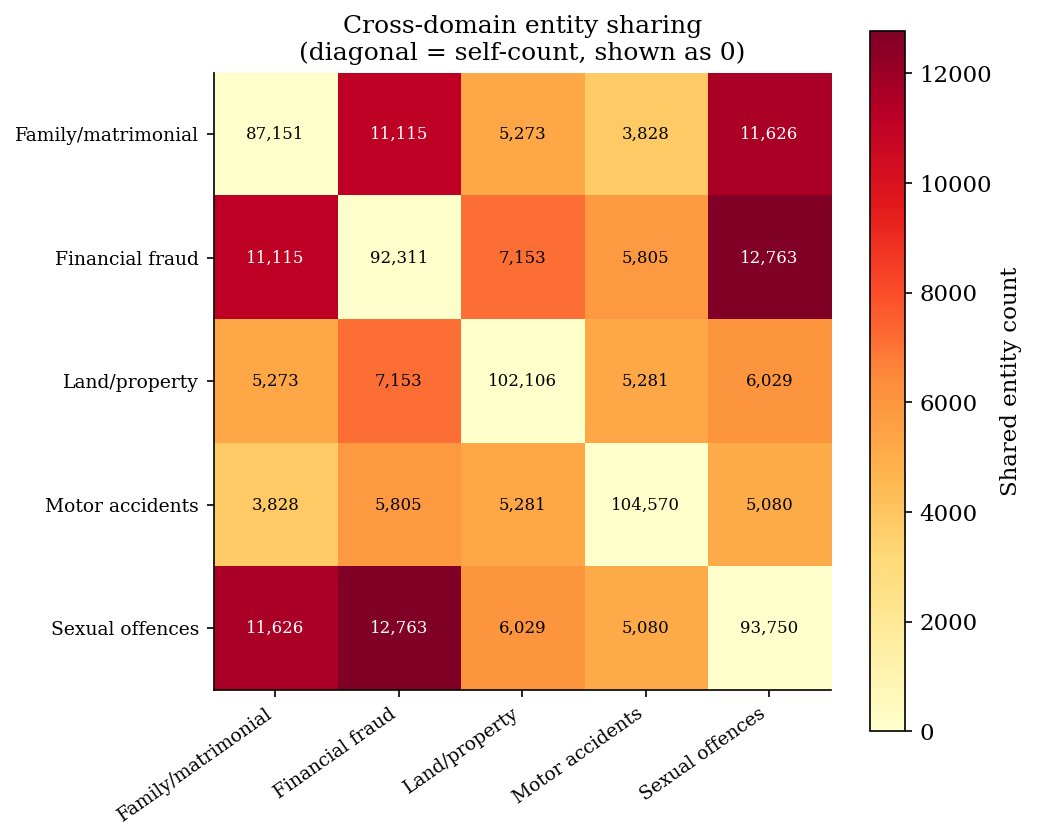
\includegraphics[width=0.9\textwidth]{figures/20_cross_bucket_sharing_matrix.png}
  \caption{Cross-bucket entity sharing matrix. Darker values indicate more shared canonicalised entities.}
  \label{fig:cross_bucket_sharing_matrix}
\end{figure}

\subsection{Connectivity Score Distribution}
\label{sec:connectivity}

A complementary question is how well each \emph{case} is wired into the shared-entity layer. A case citing hub statutes and widely-cited precedents has many high-degree shared neighbours and can receive rich aggregated information; a case sitting on rare or single-occurrence entities is structurally isolated. A \textbf{connectivity score} is assigned per case, bucket-normalised.

\begin{figure}[H]
  \centering
  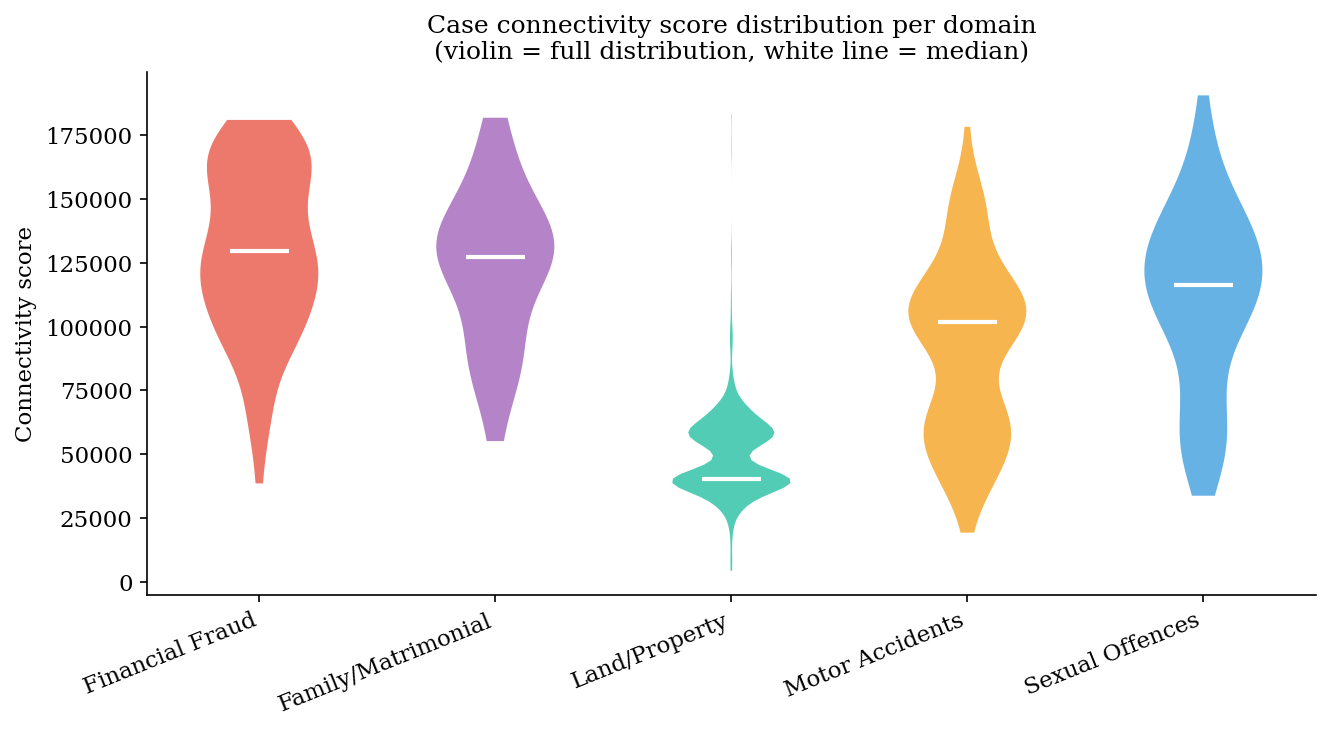
\includegraphics[width=0.9\textwidth]{figures/39_connectivity_violin.png}
  \caption{Per-bucket connectivity score distributions. Land-property and financial-fraud have wider distributions with higher medians; motor-accidents is concentrated at low connectivity.}
  \label{fig:connectivity_violin}
\end{figure}

Land-property and financial-fraud cases cite diverse authorities and are well-connected. Motor-accidents is narrow and low (repeated citation of MV Act~1988 and Section~166). Within-bucket variance is substantial: prediction difficulty is heterogeneous at the case level, not just by domain. The connectivity score is used by the Graph Visualiser to rank cases when sampling Hub-Network and Case-Connection views.

\section{Per-Domain Corpus Analysis}
\label{sec:perdomain}

\subsection{Case Length Distributions}

Case length varies substantially across buckets and directly determines how text features are constructed for the GNN.

\begin{figure}[H]
  \centering
  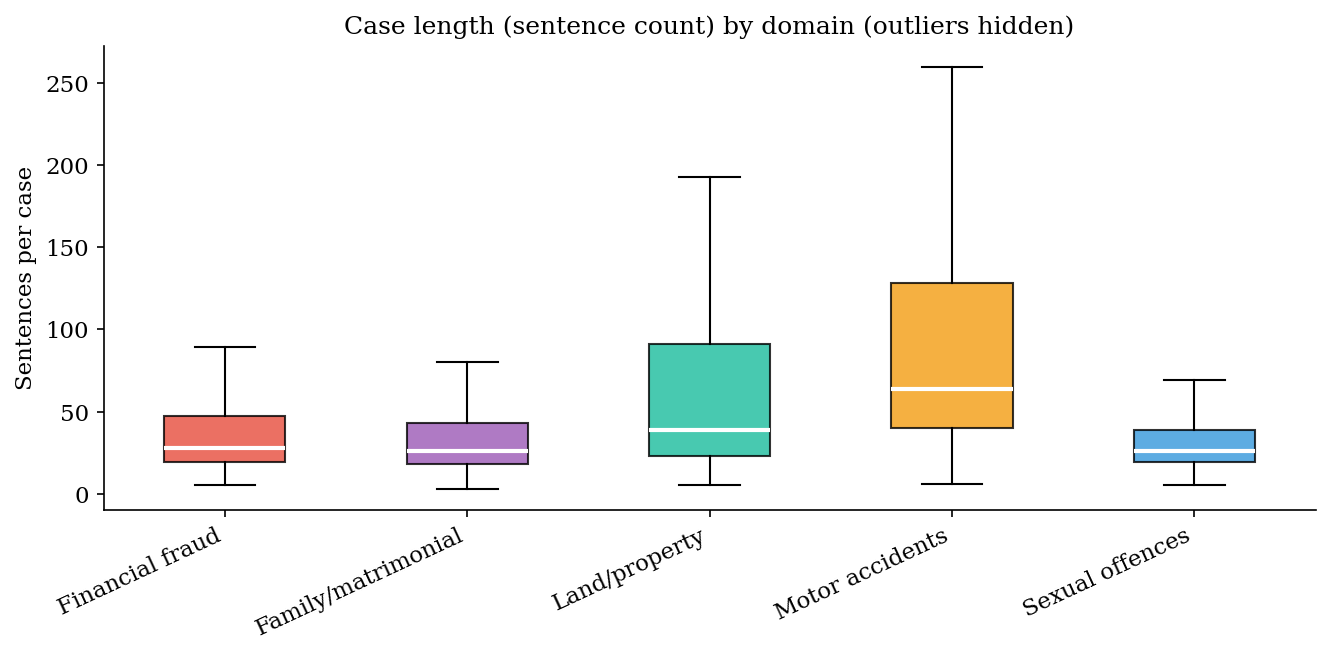
\includegraphics[width=0.92\textwidth]{figures/06_sentence_count_distribution_full.png}
  \caption{Sentence-count distribution per bucket. Land-property and financial-fraud have the heaviest right tails; motor-accidents is concentrated at low counts.}
  \label{fig:sentence_count_dist}
\end{figure}

Motor-accidents judgments are short and tribunal-style; land-property matters are long and document-heavy. These distributions drove the per-bucket hierarchical-chunking configuration in Section~\ref{sec:text_features}, with chunk boundaries set per-bucket based on the 90th-percentile sentence count.

\subsection{Entity Richness Per Domain}

Entity richness --- unique canonicalised entities per case --- predicts both graph density and modelling difficulty. Figure~\ref{fig:richness_and_degree} confirms the expected ordering: land-property and financial-fraud are entity-rich and highly connected; motor-accidents is entity-poor and low-degree.

\begin{figure}[H]
  \centering
  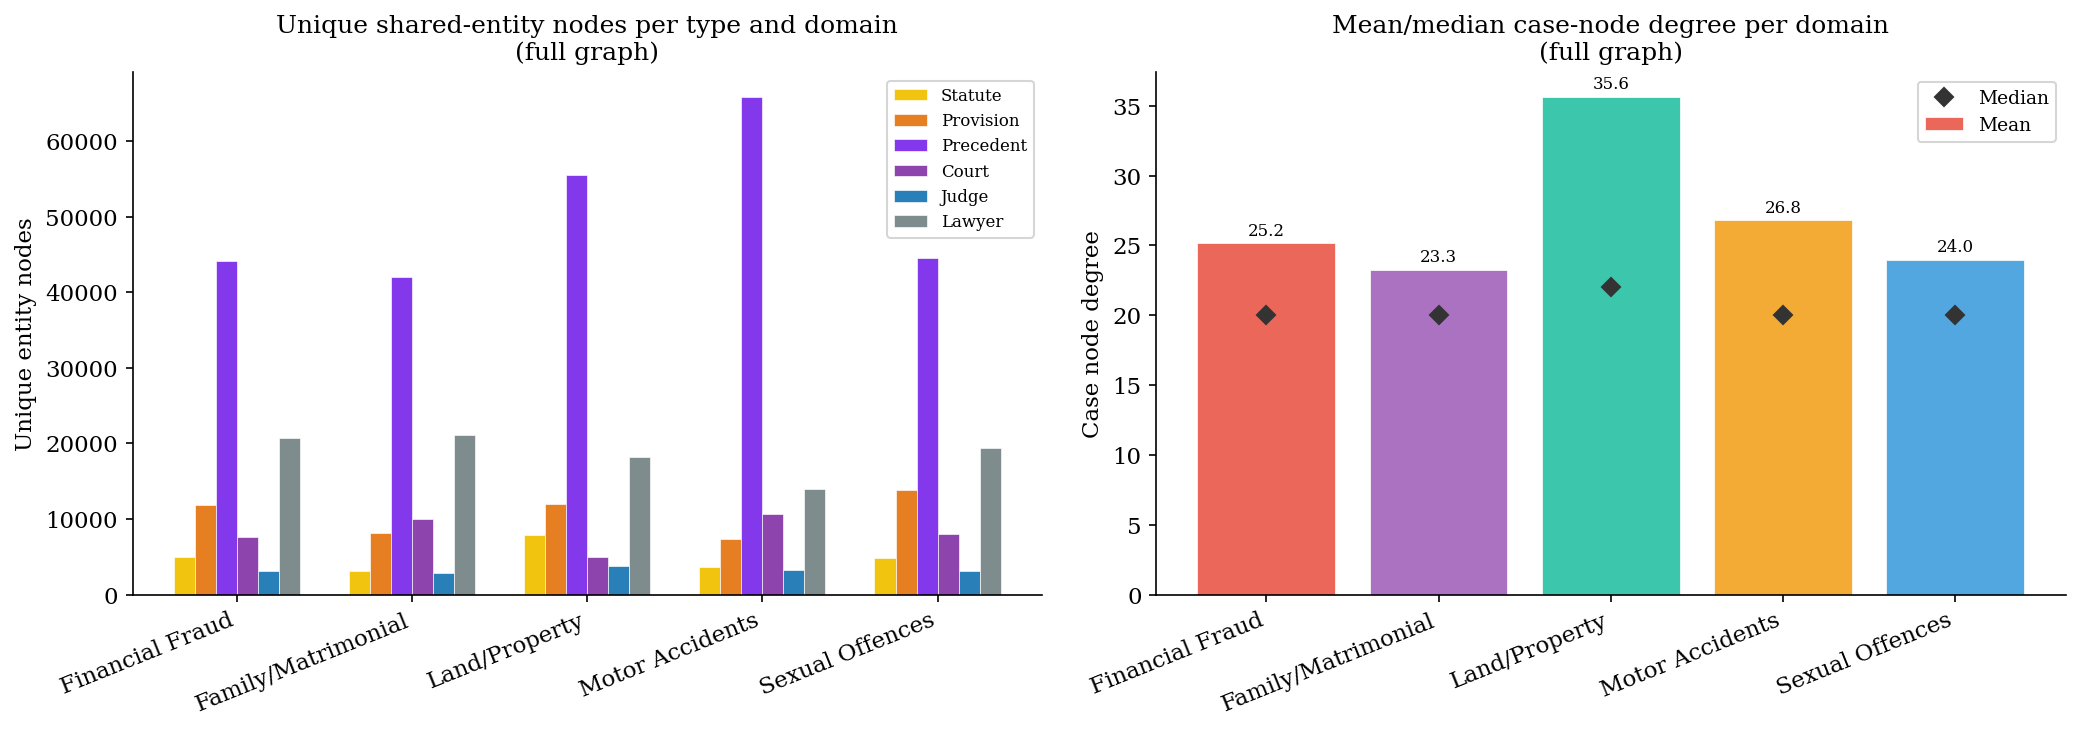
\includegraphics[width=0.92\textwidth]{figures/38_per_bucket_richness_and_degree.png}
  \caption{Entity richness and mean case degree per bucket.}
  \label{fig:richness_and_degree}
\end{figure}

The per-bucket PageRank top-5 is a near-perfect fingerprint of the underlying legal domain:
\begin{itemize}
  \item \textbf{Family \& Matrimonial}: IPC, CrPC, Sections~498A, 482.
  \item \textbf{Financial Fraud}: IPC, CrPC, Sections~420, 468, 471.
  \item \textbf{Land \& Property}: Supreme Court, Land Acquisition Act~1894, Constitution of India.
  \item \textbf{Motor Accidents}: Motor Vehicles Act~1988, Supreme Court, Apex Court, Section~166.
  \item \textbf{Sexual Offences}: IPC, CrPC, POCSO Act, Section~506.
\end{itemize}

These are exactly what a lawyer would expect --- reassuring evidence that canonicalisation and NER recover legally meaningful primary citations.

Figure~\ref{fig:within_bucket_network_fingerprints} reveals that domains differ not only in their top entities but in their network geometry. Family-matrimonial and sexual-offences share the same criminal-procedure spine but route through different specialised provisions (Section~498A vs.\ POCSO, Section~376). Land-property is multi-centred around statutory and constitutional hubs. Motor-accidents exhibits the tightest, most repetitive local backbone, leaving little diversity for multi-hop message passing to exploit.

\begin{figure}[H]
  \centering
  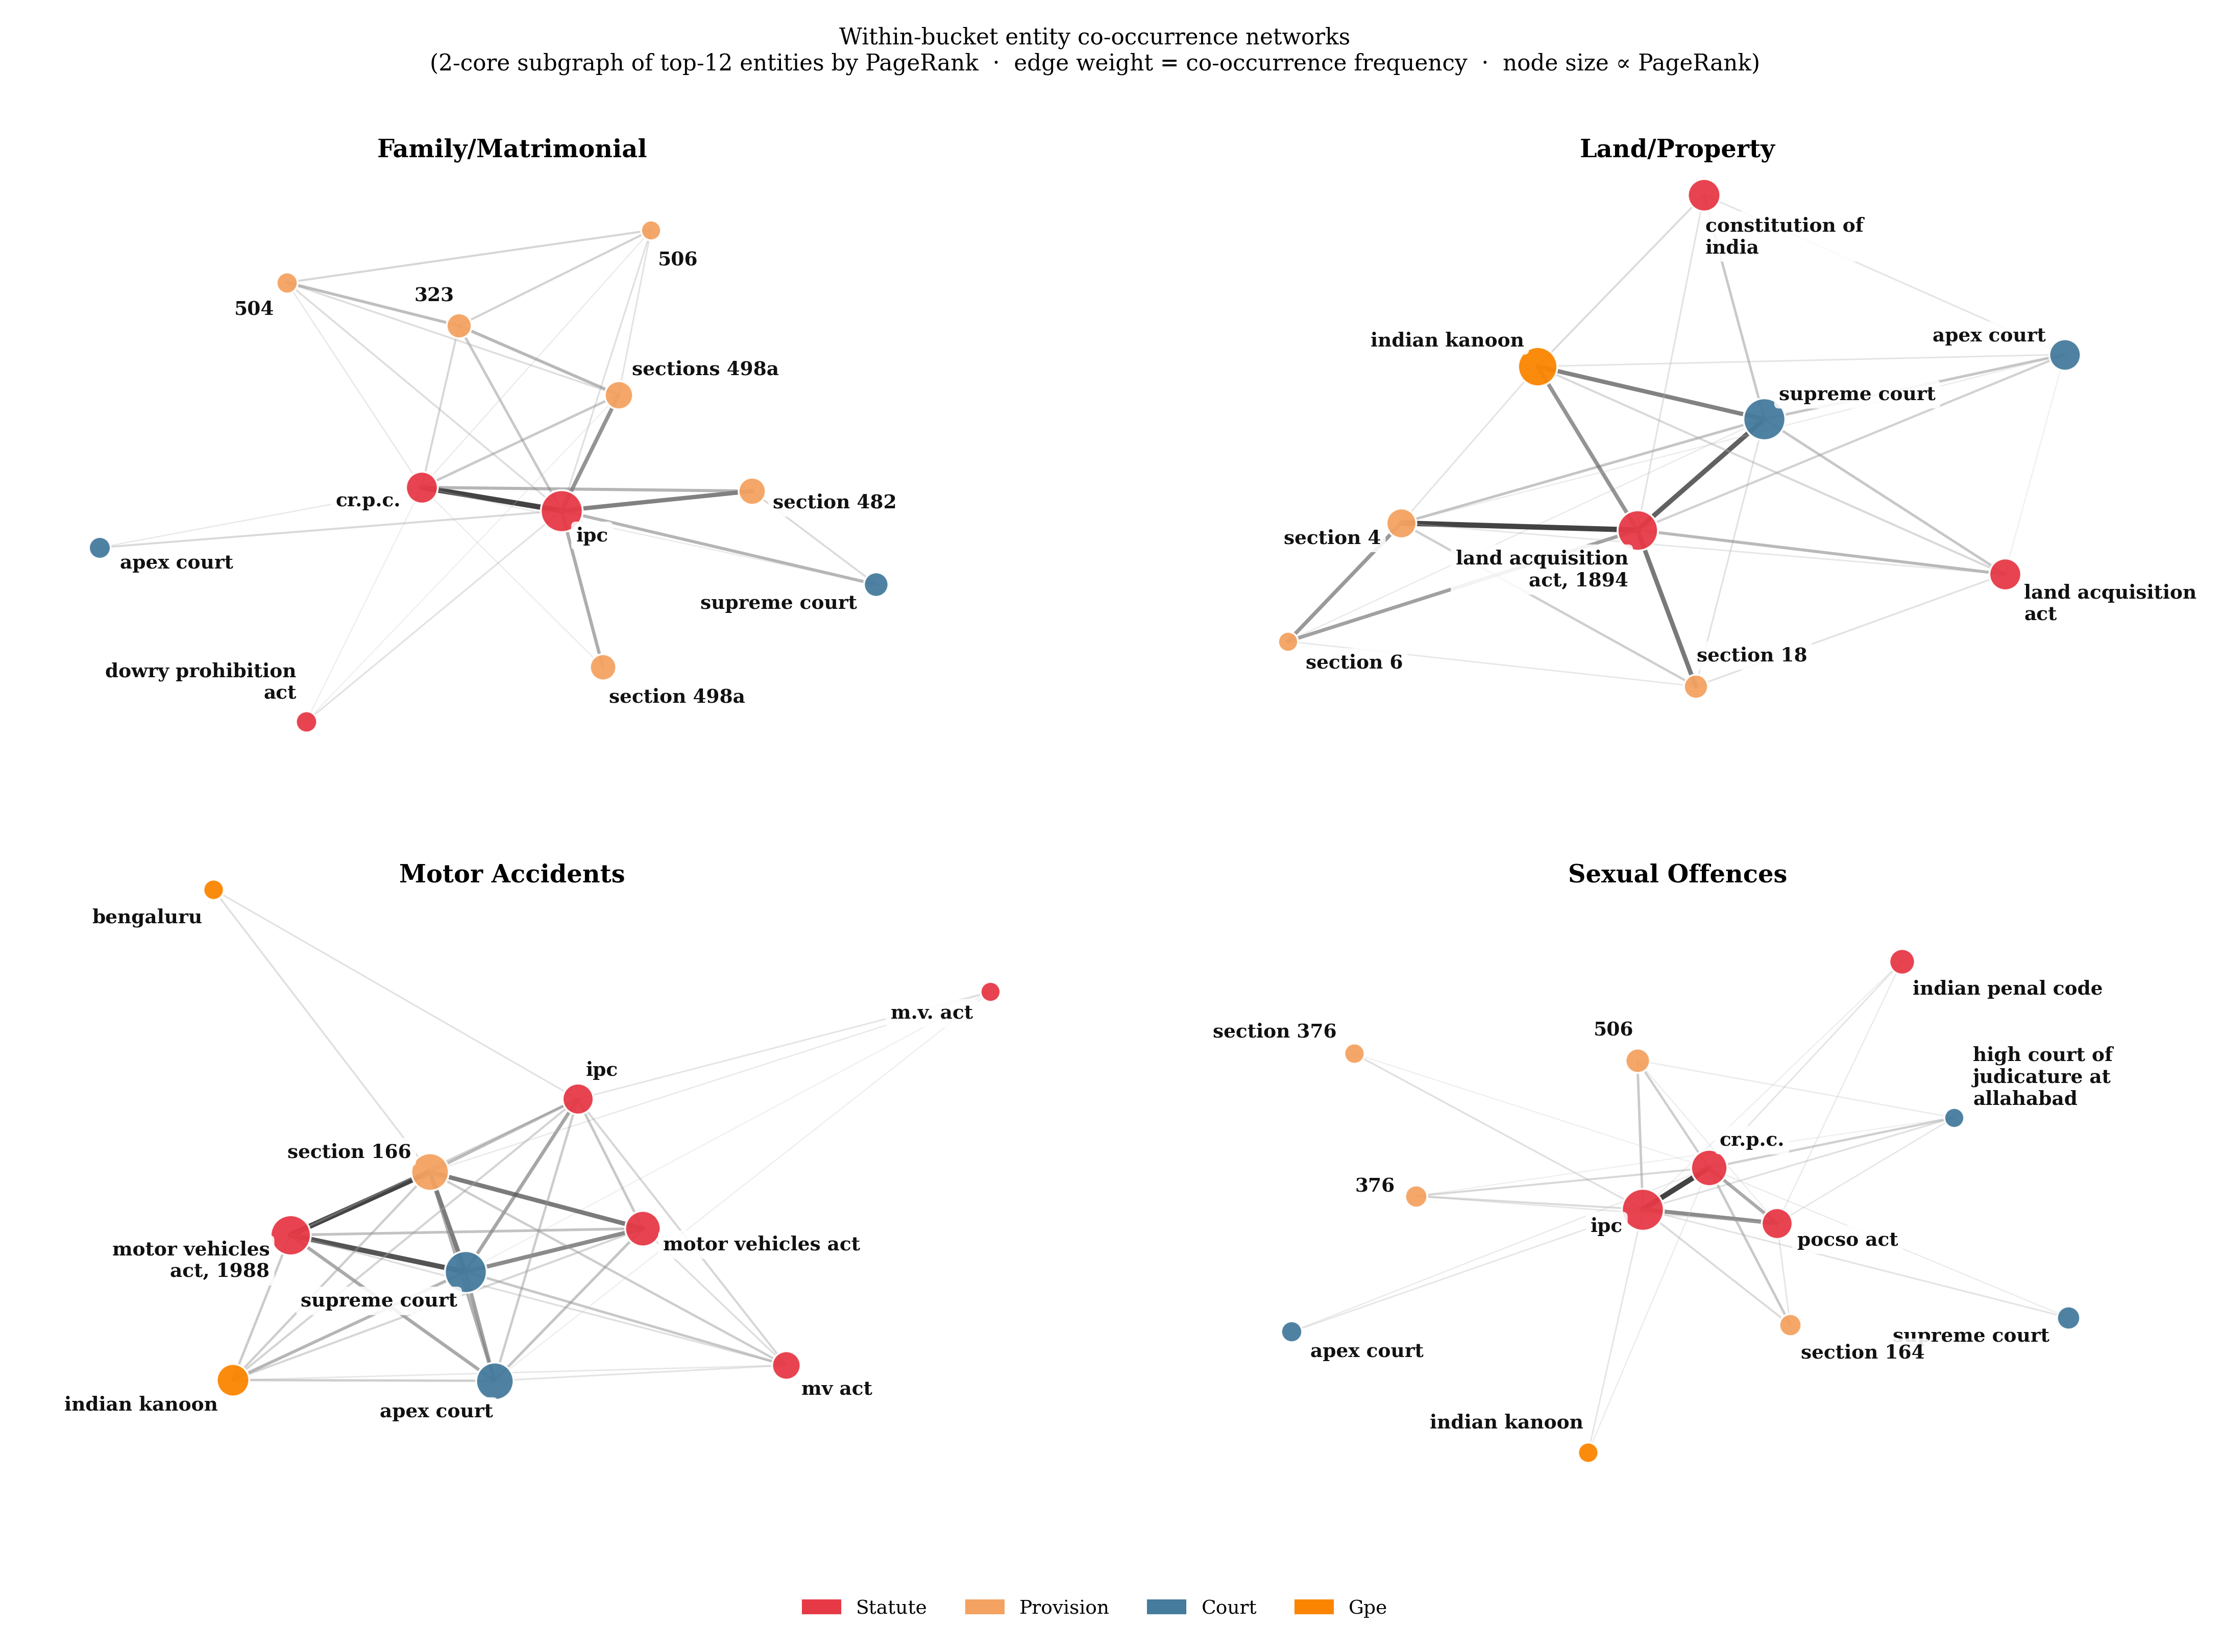
\includegraphics[width=\textwidth]{figures/36_within_bucket_network_fingerprints.png}
  \caption{Within-bucket entity co-occurrence networks for four domains, restricted to top-25 PageRank entities. Node size is proportional to PageRank.}
  \label{fig:within_bucket_network_fingerprints}
\end{figure}

Figure~\ref{fig:cross_domain_network_fingerprint} collapses all five networks into a single cross-domain view, revealing a three-tier bridge structure: \textsc{Supreme Court} and \textsc{Apex Court} appear in the top-10 of all five domains; \textsc{IPC}, \textsc{CrPC}, and \textsc{Section~482} bridge the three criminal-procedure domains; domain-exclusive entities (\textsc{Land Acquisition Act~1894}, \textsc{Motor Vehicles Act~1988}, \textsc{POCSO}) remain segregated. This stratified structure is precisely what a well-designed heterogeneous graph should exhibit: enough shared structure for cross-domain representation learning, but enough exclusivity for meaningful per-domain fingerprints.

\begin{figure}[H]
  \centering
  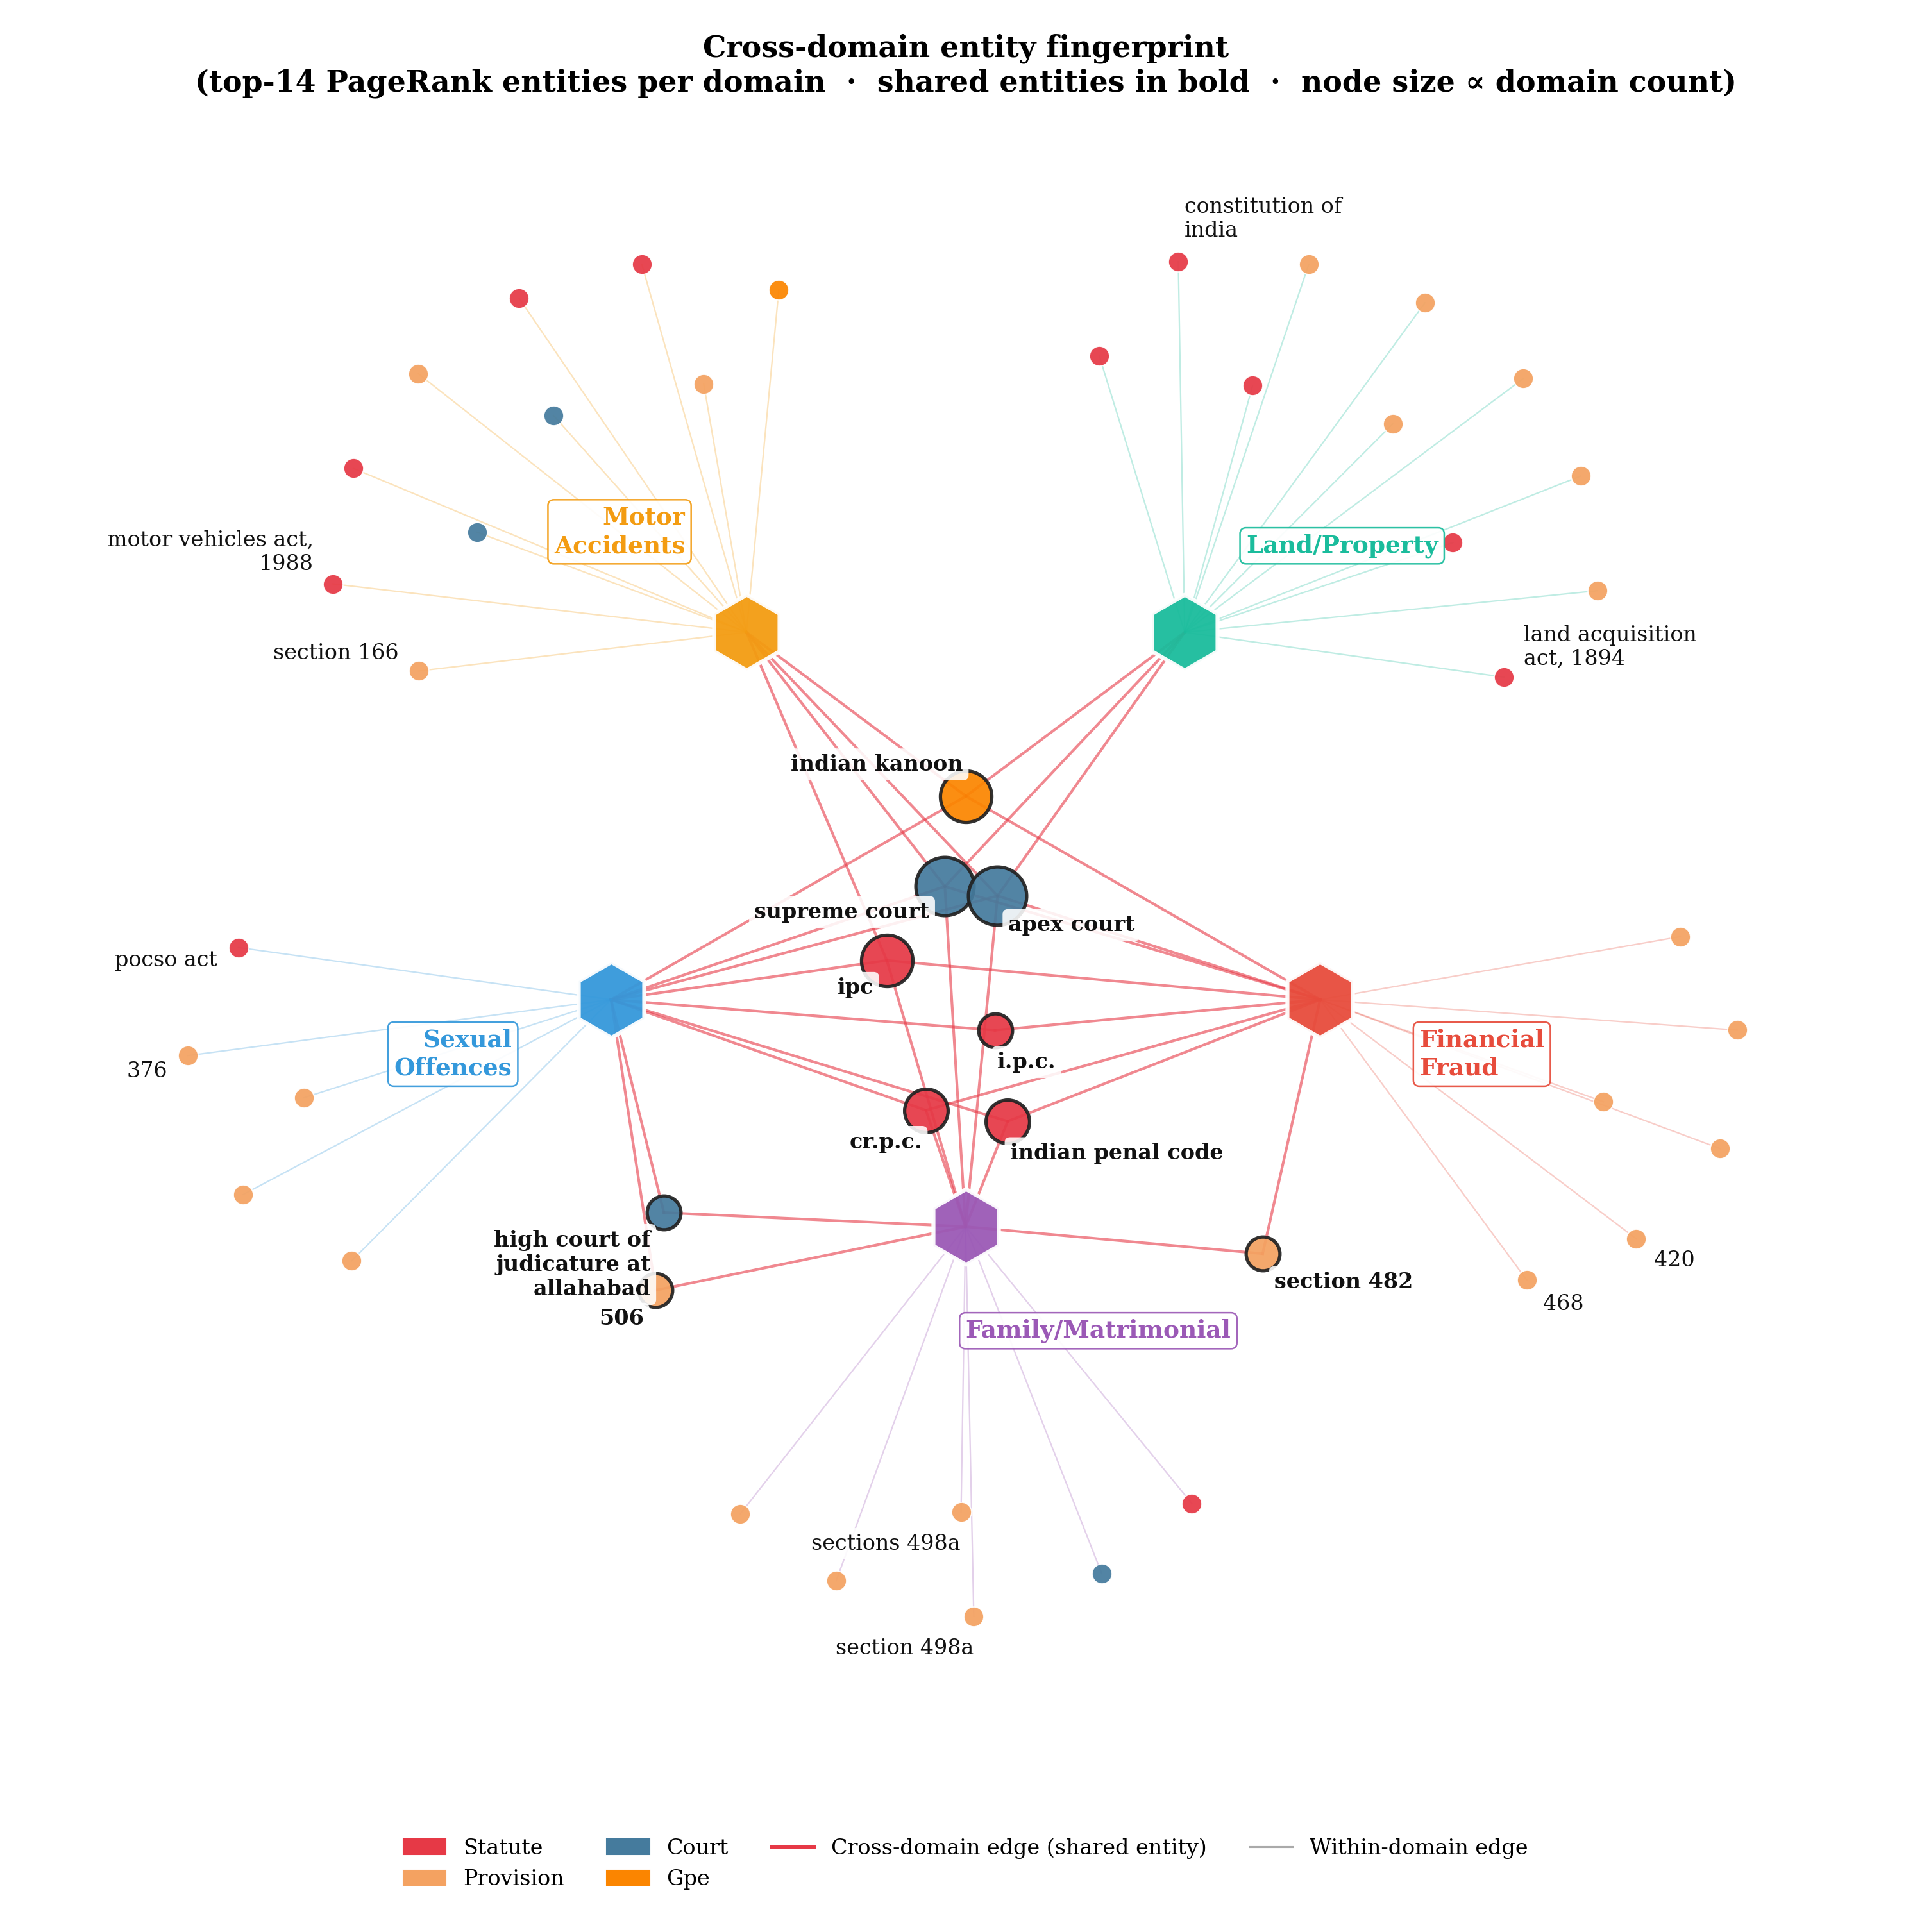
\includegraphics[width=\textwidth]{figures/44_cross_domain_network_fingerprint.png}
  \caption{Cross-domain entity fingerprint. Top-10 PageRank entities per domain around five domain-hub nodes; crimson edges connect cross-domain bridges.}
  \label{fig:cross_domain_network_fingerprint}
\end{figure}

\subsection{Rhetorical Role Composition}

Figure~\ref{fig:rr_breakdown} shows the RR breakdown after leakage-safe filtering. \textsc{RPC} and \textsc{RLC} are intentionally absent across all domains --- confirming the leakage gate works structurally, not just logically. \textsc{Facts} and \textsc{Arguments} dominate; the \textsc{Arguments} share tracks case length (largest in land-property and financial-fraud).

\begin{figure}[H]
  \centering
  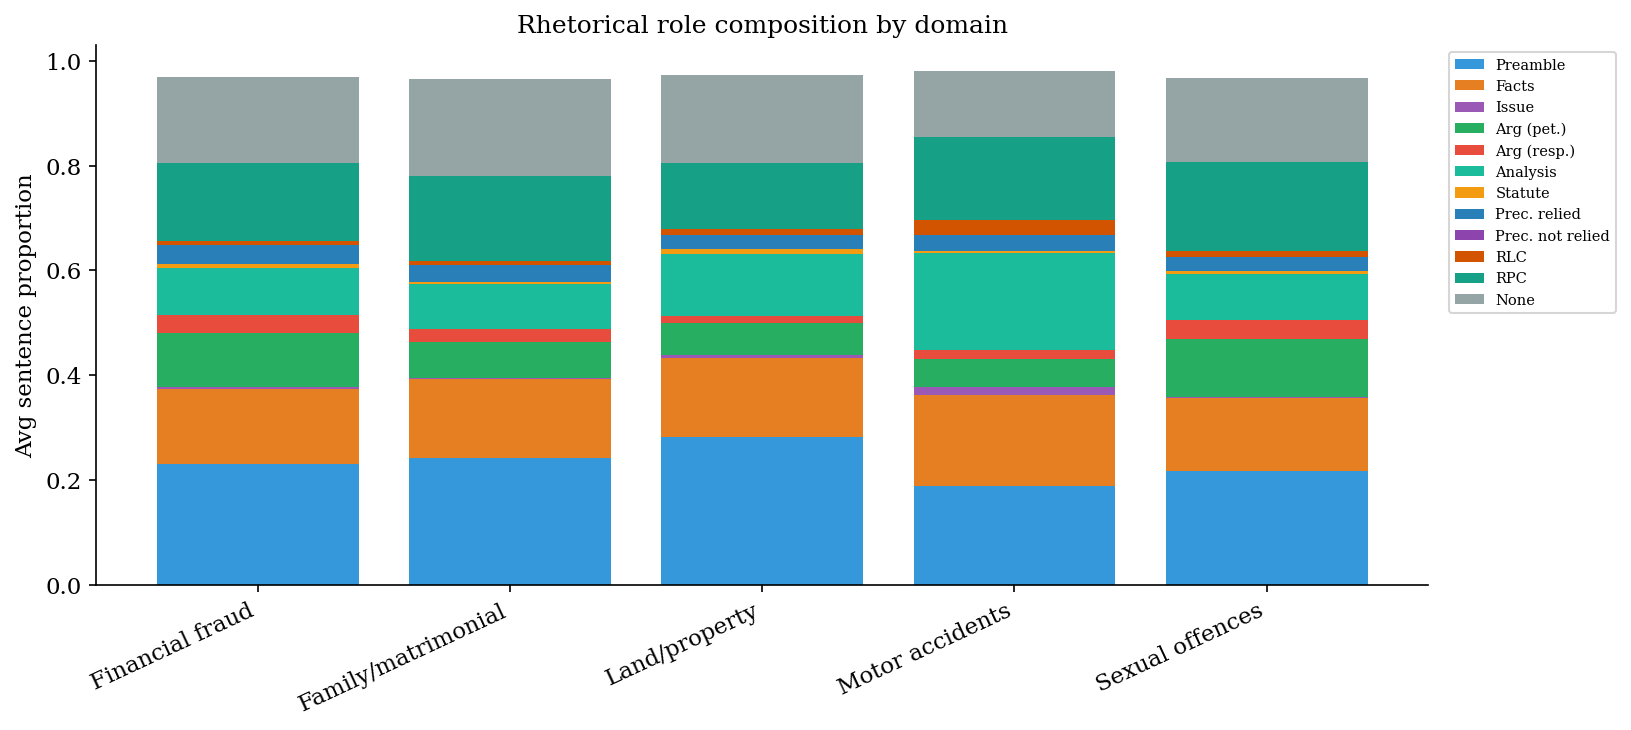
\includegraphics[width=0.95\textwidth]{figures/07_rhetorical_role_breakdown_full.png}
  \caption{Rhetorical role breakdown per bucket after leakage-safe filtering. \textsc{RPC} and \textsc{RLC} are absent across all domains.}
  \label{fig:rr_breakdown}
\end{figure}

\section{Key Structural Insights}
\label{sec:key_insights}

\begin{enumerate}
  \item \textbf{Hub-dominated.} A small set of cross-bucket statutes and courts (IPC, CrPC, Supreme Court) forms the spine; most other entities are long-tail leaves.
  \item \textbf{Cross-domain sharing is real but uneven.} The four IPC/CrPC-driven buckets share heavily; land-property partially detaches via its own statutory backbone.
  \item \textbf{Identity-proxy leakage is structural.} Judges, specific lawyers, and specific courts have bridge scores high enough to make sharing them across cases unsafe --- vindicating the decision to hold them local.
  \item \textbf{Connectivity score predicts modelling difficulty.} Low-connectivity cases have fewer shared-entity neighbours to aggregate from.
  \item \textbf{The per-domain fingerprints are legally coherent} --- the strongest evidence that NER, canonicalisation, and RR filtering together produce a legally faithful corpus.
\end{enumerate}
